\documentclass{article}
\usepackage[top=50pt,bottom=42pt,left=50pt,right=48pt]{geometry}

\usepackage[slovene]{babel}
\usepackage{amsmath}
\usepackage{color}
%\usepackage{graphicx,subfigure}

%\usepackage{subfigure}

\usepackage[T1]{fontenc}
\usepackage[utf8]{inputenc}
\usepackage{lmodern}
\usepackage{amsmath}
\usepackage{tikz}
\usetikzlibrary{shapes,shapes.geometric,arrows,fit,calc,positioning,automata}

\usepackage{amsfonts}
\usepackage{mathrsfs}

\usepackage{float}

\usepackage{caption}
\usepackage{subcaption}

%\usepackage{chemformula}
%\usepackage[version=4]{mhchem}
%\usepackage{mychemistry}
%\usepackage{chemfig}

%\def\phi{\varphi}
%\def\eps{\varepsilon}
%\def\theta{\vartheta}

%\usepackage{physics} ta je za vektorje: \vectorbold{}

\newcommand{\thisyear}{2020/21}

\renewcommand{\Re}{\mathop{\rm Re}\nolimits}
\renewcommand{\Im}{\mathop{\rm Im}\nolimits}
\newcommand{\Tr}{\mathop{\rm Tr}\nolimits}
\newcommand{\diag}{\mathop{\rm diag}\nolimits}
\newcommand{\dd}{\,\mathrm{d}}
\newcommand{\ddd}{\mathrm{d}}
\newcommand{\ii}{\mathrm{i}}
\newcommand{\lag}{\mathcal{L}\!}
\newcommand{\ham}{\mathcal{H}\!}
\newcommand{\four}[1]{\mathcal{F}\!\left(#1\right)}
\newcommand{\bigO}[1]{\mathcal{O}\!\left(#1\right)}
\newcommand{\sh}{\mathop{\rm sinh}\nolimits}
\newcommand{\ch}{\mathop{\rm cosh}\nolimits}
\renewcommand{\th}{\mathop{\rm tanh}\nolimits}
\newcommand{\erf}{\mathop{\rm erf}\nolimits}
\newcommand{\erfc}{\mathop{\rm erfc}\nolimits}
\newcommand{\sinc}{\mathop{\rm sinc}\nolimits}
\newcommand{\rect}{\mathop{\rm rect}\nolimits}
\newcommand{\ee}[1]{\cdot 10^{#1}}
\newcommand{\inv}[1]{\left(#1\right)^{-1}}
\newcommand{\invf}[1]{\frac{1}{#1}}
\newcommand{\sqr}[1]{\left(#1\right)^2}
\newcommand{\half}{\frac{1}{2}}
\newcommand{\thalf}{\tfrac{1}{2}}
\newcommand{\pd}{\partial}
\newcommand{\Dd}[3][{}]{\frac{\ddd^{#1} #2}{\ddd #3^{#1}}}
%\newcommand{\Pd}[3][{}]{\frac{\pd^{#1} #2}{\pd #3^{#1}}}
\newcommand{\avg}[1]{\left\langle#1\right\rangle}
\newcommand{\norm}[1]{\left\Vert #1 \right\Vert}
\newcommand{\braket}[2]{\left\langle #1 \vert#2 \right\rangle}
%\newcommand{\obraket}[3]{\left\langle #1 \vert #2 \vert #3 \right \rangle}
%\newcommand{\hex}[1]{\texttt{0x#1}}
\newcommand{\vect}[1]{\boldsymbol{#1}}

\renewcommand{\iint}{\mathop{\int\mkern-13mu\int}}
\renewcommand{\iiint}{\mathop{\int\mkern-13mu\int\mkern-13mu\int}}
\newcommand{\oiint}{\mathop{{\int\mkern-15mu\int}\mkern-21mu\raisebox{0.3ex}{$\bigcirc$}}}

\newcommand{\wunderbrace}[2]{\vphantom{#1}\smash{\underbrace{#1}_{#2}}}

\renewcommand{\vec}[1]{\overset{\smash{\hbox{\raise -0.42ex\hbox{$\scriptscriptstyle\rightharpoonup$}}}}{#1}}
\newcommand{\bec}[1]{\mathbf{#1}}



\begin{document}



\begin{titlepage}
\begin{center}
	
	{\sc\Large	Simetrije v fiziki}\\
	\vspace*{5cm}
	\Large\textbf{Spontani zlom simetrije}\\
	\vspace{0.2cm}
	\vspace{1.6cm}
	\largeŽan Butala\\
	\text{vpisna številka: 28222060}
 
      % \vspace{1cm}
	%\begin{figure}[H]
   %	 \centering
    %	\includegraphics[width=10cm]{semafor1.png}
    	%\label{fig:graf1}
	%\end{figure}
       \vfill 

	\normalsize
 
       {\sc 15. december 2023\\
	\vspace{0.2cm}
       Univerza v Ljubljani\\
       Fakulteta za matematiko in fiziko\\}
      
\end{center}
\end{titlepage}


\newpage


\section{Globalna simetrija}

Spontani zlom simetrije, Nambu-Goldstone-ov izrek. Literatura: Gauge theory of elementary particle physics, T-P. Cheng and L-F. Li (pages 144-145).

Spontani zlom SU(2)LX SU(2)R kiralna simetrija, sigma model.

Pioni kot  Nambu-Goldstone-ov bozoni, mase nukleonov. mass of nucleon. Literatura: Gauge theory of elementary particle physics, T-P. Cheng and L-F. Li, 144-150;


\begin{figure}[H]
     \centering
     \begin{subfigure}[b]{0.47\textwidth}
        \hspace*{-5mm}
         \centering
         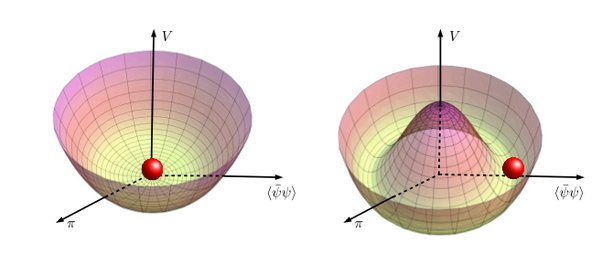
\includegraphics[width=1.0\textwidth]{spont2.jpg}
         \caption{Brez pomnoževanja.}
         \label{fig:expa}
     \end{subfigure}
     \begin{subfigure}[b]{0.47\textwidth}
       \hspace*{+3mm}
         \centering
         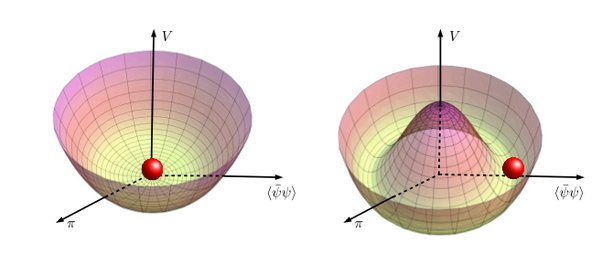
\includegraphics[width=1.0\textwidth]{spont2.jpg}
         \caption{Pomnoževanje; variiramo $t_{zač}$ in $t_{konč}$.}
         \label{fig:expb}
     \end{subfigure}
        \caption{Napoved elastičnih konstant iz eksperimentalnih meritev.}
        \label{fig:exp}
\end{figure}


\begin{figure}[H]
    \hspace*{-0.1cm}
    \centering
    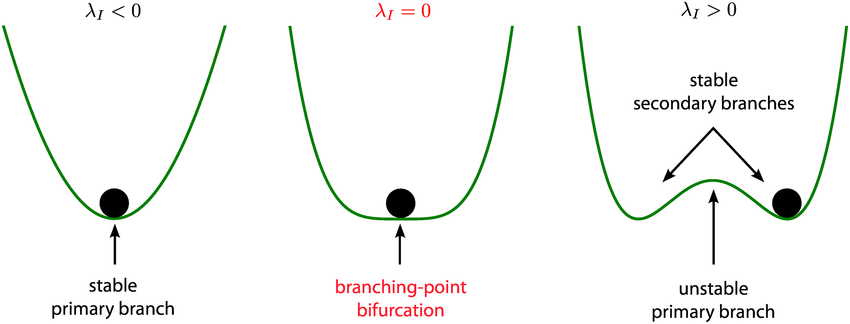
\includegraphics[height=5.5cm]{spont1.png}
    \caption{Abc.}
    \label{fig:exp2}
\end{figure}


\begin{thebibliography}{9}
\bibitem{texbook}
F. Halzen in A. D. Martin 
\emph{Quarks and Leptons: An Introductory Course in Modern Particle Physics.} Wiley, 1984

\bibitem{texbook}
Michael E. Peskin \emph{The \TeX{} Book}, Addison-Wesley Professional.
An Introduction to quantum field theory.
CRC press, 2018.

\bibitem{texbook}
Why do we expect a Higgs boson? Part I: Electroweak Symmetry Breaking \emph{The \TeX{} Book}, Addison-Wesley Professional.
url: http://www.quantumdiaries.org/2011/11/21/why-do-we-expecta-higgs-boson-part-i-electroweak-symmetry-breaking/.

\bibitem{lamport94}
Leslie Lamport (1994) \emph{\LaTeX: a document preparation system}, Addison
Wesley, Massachusetts, 2nd ed.
\end{thebibliography}

\end{document}